\lab{Петля гистерезиса (динамический метод)}
\label{lab:4-5}

\aim{изучение петель гистерезиса различных ферромагнитных мате­риалов
    в переменных полях.}

\equip{автотрансформатор, понижающий транс­форматор, интегрирующая цепочка,
амперметр, вольтметр, элек­тронный осциллограф, делитель напряжения,
тороидальные образцы с двумя обмотками.}

Перед выполнением работы необходимо ознакомиться с
пп.~\ref{sec:ferromagnetism}, \ref{sec:histeresis} и~\ref{sec:measure-HB} 
теоретического Введения к разделу.


Ферромагнитные материалы часто применяются в трансформаторах, дросселях, машинах
переменного тока, то есть в устройствах, где они подвергаются периодическому
перемагничиванию, --- поэтому изучение магнитных характеристик 
ферромагнетиков в переменных полях представляет большой практический интерес. 
Основные характеристики ферромагнетиков~--- их коэрцитивное поле
$H_c$, магнитная проницаемость $\mu$, 
рассеиваемая в виде тепла при перемагничивании мощность~--- зависят
от частоты перемагничивающего поля. В данной работе
кривые гистерезиса ферромагнитных материалов изучаются в поле частоты
$\nu_0 = 50~Гц$ с помощью электронного осциллографа.

\begin{figure}[h!]
    %     \hfil\pic{0.38\textwidth}{4_4_1}
    \centering
    \pic{62mm}{Chapter_4/4-4-hist}
    \caption{Петля гистерезиса ферромагнетика}
    \figmark{loop}
\end{figure}

Магнитная индукция~${B}$ и напряжённость поля~${H}$ в~ферромагнитном материале 
неоднозначно связаны между собой: индукция зависит не только от напряжённости, 
но и от предыстории образца. Связь между~$B$ и~$H$ типичного ферромагнетика 
иллюстрирует рис.~\figref{loop}.


Если к ферромагнитному образцу прикладывать переменное внешнее магнитное поле,
то его состояние на плоскости $H$--$B$ будет изменяться по замкнутой кривой~---
\emph{петле гистерезиса}. Размер петли определяется максимальным
значением напряжённости~$H$ в цикле (напр.,
петля AA$'$, обозначенная пунктиром на рис. \figref{loop}). 
Если амплитуда напряжённости достаточно
велика, то образец будет периодически достигать \emph{насыщения}, 
что на рисунке соответствует кривой CEFC$'$E$'$F$'$C
(\emph{предельная петля гистерезиса}).
Пересечение предельной петли с вертикальной осью соответствует
остаточной индукции~$B_r$, пересечение с горизонтальной осью ---
коэрцитивному полю~$H_c$.
Крайние точки петель, соответствующие амплитудным значениям~$H$ 
(например, точка~A на рис.~\figref{loop}), лежат на 
\emph{начальной кривой намагничивания}~(OAC).

\paragraph{Измерение магнитной индукции}
Магнитную индукцию $B$ удобно определять с
помощью ЭДС, возникающей при изменении магнитного потока $\Phi$ в катушке,
намотанной на образец.
Пусть катушка c $N$ витками плотно охватывает образец сечением $S$, и индукция $B$ в образце однородна.
Из формулы \chaptereqref{EMF-magnetic flux}
имеем
%
%  В
% этом случае
% \begin{equation}
% 	\eqmark{4.5.1}
% 	\Phi = BSN_k.
% \end{equation}
%
% Тогда при изменении магнитного потока ЭДС в катушке будет равна
% \begin{equation*}
% 	\mathcal{E} = -\frac{d\Phi}{dt} = -SN_k\frac{dB}{dt},
% \end{equation*}
% и
\begin{equation}
	\eqmark{4.5.2}
	|B| = \frac{1}{SN}\int \mathcal{E}dt.
\end{equation}
Таким образом, для определения $B$ нужно проинтегрировать сигнал, 
наведённый меняющимся магнитным полем в измерительной катушке, 
намотанной на образец.

\begin{wrapfigure}{r}{0.42\textwidth}
\centering
    \pic{\linewidth}{Chapter_4/4_5_1}
    \caption{Интегрирующая цепочка}
    \figmark{integrating curcuit}
\end{wrapfigure}
Для интегрирования в работе используется
\emph{интегрирующая} $RC$-цепочка (рис.~\figref{integrating curcuit}).
<<Входное>> напряжение от источника $U_{вх}(t)$ подаётся на последовательно соединённые
резистор~$R$ и конденсатор~$C$.
<<Выходное>> напряжение $U_{вых}(t)$ снимается с конденсатора.
Предположим, что 1) сопротивление источника мало по сравнению с $R$: $R_{ист}\ll R$,
2) выходное сопротивление (сопротивление на входе осциллографа),
напротив, велико: $R_{вых}\gg R$ и, наконец,
3) сопротивление $R$ достаточно велико, так что почти всё падение напряжения
приходится на него, а $U_{вых}\ll U_{вх}$.
В таком случае ток цепи равен $I=(U_{вх}-U_{вых})/R\approx U_{вх}/R$, и
входное и выходное сопротивление связаны соотношением
\begin{equation}
	\eqmark{4.5.3}
% 	\begin{aligned}
    U_\text{вых} = \frac{q}{C} =\frac{1}{C}\int\limits_0^t Idt
\approx \frac{1}{R C}\int\limits_0^t U_\text{вх} dt.
% Это просто неправильно! // ППВ
%     \frac{1}{C}\int \frac{U_\text{вх}}{\sqrt{R^2 + \frac{1}{(\omega C)^2}}}
%     \frac{dt}{\omega C}
% =
% 		= \frac{1}{RC}&\int \frac{U_\text{вх}}{\sqrt{1 + \frac{1}{(\omega
% RC)^2}}} dt
% 	\end{aligned}
\end{equation}
Для индукции поля из \eqref{4.5.2} получаем
\begin{equation}
    \eqmark{4.5.4}
    |B| = \frac{1}{SN}\int U_\text{вх}dt =
\frac{RC}{SN}U_\text{вых}.
\end{equation}

Уточним критерий применимости соотношения \eqref{4.5.3}.
Пусть на вход интегрирующей ячейки подан синусоидальный сигнал
с частотой~$\omega_0$. Тогда, пользуясь методом комплексных амплитуд, нетрудно найти
отношение амплитуд входного и выходного напряжений:
\begin{equation*}
\frac{U_{вых}}{U_{вх}} = \frac{1/(\omega_0 C)}{\sqrt{R^2+\frac{1}{(\omega_0 C)^2}}}.
\end{equation*}
Видно, что неравенство $U_{вых}\ll U_{вх}$ реализуется,
если
\begin{equation}
    R\gg \frac{1}{\omega_0 C}
\end{equation}
(импеданс конденсатора мал по сравнению
сопротивлением резистора). 
%Это же соотношение можно переписать как
%$T_0 \ll \tau_C$, где $T_0$ --- период колебаний, $\tau_C=RC$ --- характерное
%время разрядки конденсатора.
В таком случае для синусоидального сигнала имеем
\begin{equation}
    \eqmark{4.5.5}
    \frac{U_{вых}}{U_{вх}} \approx \frac{1}{\omega_0 R C}.
\end{equation}

В общем случае, если $\omega_0$ --- частота самой низкой гармоники в спектре произвольного
входного сигнала, то при $\omega_0 R C\gg1$ неравенство $U_{вых}\ll U_{вх}$ выполняется
на любой частоте $\omega>\omega_0$.


% , где $\omega_0$ --- частота самой низкой
% гармоники сигнала (частота повторения $\omega_0 = 2\pi \nu_0$),
% выходное напряжение ячейки будет пропорционально интегралу от входного.
% , и здесь $\omega$~--- частота самой низкой
% гармоники~--- частота повторения $\omega = 2\pi/T.$



\experiment

Схема установки изображена на рис.~\figref{experimental environment}.
Напряжение сети (220~В, 50~Гц) с помощью трансформаторного блока~Т,
состоящего из регулировочного автотрансформатора
и разделительного понижающего трансформатора, подаётся на намагничивающую
обмотку~$N_0$ исследуемого образца.

В цепь намагничивающей катушки, на которую подаётся некоторое напряжение
$U_0$, последовательно включено сопротивление $R_0$.
Напряжение на $R_0$, равное $U_R=R_0I_0$, где $I_0$ --- ток в
намагничивающей обмотке~$N_0$, подаётся на канал~$X$ осциллографа.
Связь напряжённости~$H$ в образце и тока~$I_0$ рассчитывается по теореме
о циркуляции (см.~\chaptereqref{H-toroid}).
\important{Действующее} значение переменного тока в обмотке~$N_0$ 
измеряется амперметром~$A$.

Для измерения магнитной индукции~$B$ с измерительной обмотки~$N_{и}$ на
вход $RC$-цепочки подаётся напряжение $U_{и}$ ($U_{вх}$),
пропорциональное производной~$dB/dt$.
С~интегрирующей ёмкости~$C_{и}$ снимается напряжение~$U_C$ ($U_{вых}$),
пропорциональное величине~$B$, и подаётся на вход~$Y$ осциллографа.
Значение индукции поля~$B$ рассчитывается по формуле
\eqref{4.5.4}.

\begin{figure}[h!]
\centering
 	\pic{\textwidth}{Chapter_4/4-5-exp}
%    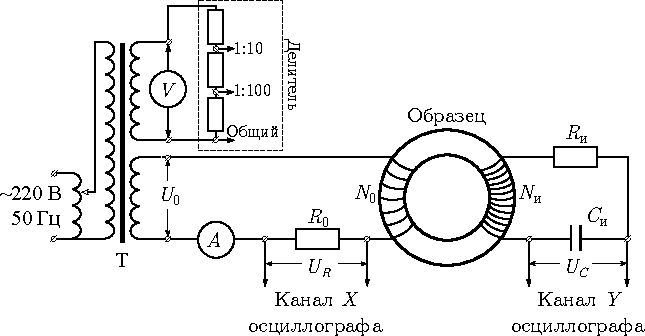
\includegraphics[width=\textwidth]{Chapter_4/4-5-exp.pdf}
	\caption{Схема установки для исследования намагничивания образцов}
	\figmark{experimental environment}
\end{figure}

Замкнутая кривая, возникающая на экране, воспроизводит в некотором масштабе
(различном для осей $X$ и $Y$) петлю гистерезиса. Чтобы придать этой кривой
количественный смысл, необходимо установить масштабы изображения, т. е. провести
калибровку каналов~$X$ и~$Y$ осциллографа.
% Для этого, во-первых, надо узнать,
% каким напряжениям (или токам) соответствуют амплитуды сигналов, видимых на экране, и,
% во-вторых, каким значениям~$B$ и~$H$ соответствуют эти напряжения (или токи).
%
% Значения напряжённости поля~$H$ пропорционально току~$I_0$ в намагничивающей
% катушке $N_0$ (а значит напряжению~$U_R=I_0 R_0$ на резисторе $R_0$)
% и рассчитывается по теореме о циркуляции (см.~\chaptereqref{H-toroid}).



% Напряжение, пропорциональное току в намагничивающей обмотке, подаётся на
% горизонтальную ось $X$.
% Если ручка усиления оси $X$ в положении калибр, цену
% деления по горизонтальной оси получим, разделив цену деления в вольтах
% на сопротивление $R_0$ в амперах.

% Для дополнительной проверки с помощью амперметра нужно закоротить обмотку $N_0$.

Калибровка канала~$X$ осциллографа производится с помощью амперметра $A$.
Предварительно необходимо закоротить обмотку $N_0$
(так как катушка с ферромагнитным образцом является
нелинейным элементом, ток в ней не имеет синусоидальной формы,
поэтому связать амплитуду тока с показаниями амперметра можно лишь
с довольно большой погрешностью). При закороченной обмотке $N_0$
показания эффективного тока, умноженные на $2\sqrt{2}$,
дадут значение удвоенной амплитуды тока, подаваемого на ось $X$,
соответствующего ширине горизонтальной развёртки на экране
(осциллограф должен работать в режиме $X$--$Y$).

Калибровка вертикальной оси~$Y$, как правило, не нужна
(переключатель масштабов осциллографа откалиброван при изготовлении ---
при условии, что ручка плавной регулировки находится в положении
калибровки). Тем не менее, она может проводиться с помощью сигнала,
снимаемого через делитель напряжения со второй катушки понижающего трансформатора
(рис.~\figref{experimental environment}). Вольтметр $V$ может достаточно точно
измерить эффективное напряжение, подаваемое на вход осциллографа. После
этого можно сравнить показания осциллографа и вольтметра.


Постоянную времени $RC$-цепочки можно определить экспериментально.
С обмотки $U_0$ на вход интегрирующей цепочки подаётся синусоидальное напряжение
с частотой цепи $\nu_0=\frac{\omega_0}{2\pi}=50\;Гц$.
На вход $Y$ осциллографа или цифрового вольтметра поочерёдно
подаются сигналы со входа ($U_\text{вх}=U_0$) и выхода ($U_\text{вых} = U_C$)
$RC$-цепочки. Измерив амплитуды этих сигналов, можно рассчитать постоянную
времени $\tau_C= RC$ по формуле \eqref{4.5.5}.
Кроме того, сопротивление и ёмкость можно независимым образом измерить
цифровым мультиметром.
% \begin{equation}
% 	\eqmark{4.5.6}
% 	RC = \frac{U_\text{вх}}{\omega U_\text{вых}}
% \end{equation}

\begin{lab:task}

\taskpreamble{В работе предлагается при помощи электронного осциллографа
исследовать предельные петли гистерезиса и
начальные кривые намагничивания для нескольких ферромагнитных образцов;
определить магнитные характеристики материалов, чувствительность каналов $X$ и
$Y$ осциллографа и постоянную времени $\tau$ интегрирующей цепочки.}

\tasksection{Измерение петли гистерезиса}

\item
Для наблюдения петли гистерезиса на экране электронного осциллографа~(ЭО)
соберите схему согласно рис.~\figref{experimental environment}. 
Подготовьте приборы к работе.

\item
Подберите ток питания в намагничивающей обмотке и коэффициен­ты усиления ЭО так,
чтобы предельная петля гистерезиса занимала большую часть экрана (при этом
ширина петли при увеличении тока практически не меняется).

\item
Зафиксируйте (сфотографируйте или зарисуйте на кальку)
предельную петлю гистерезиса и оси координат; отметьте на осях деления
шкалы. Запишите материал образца, значения коэффициентов усиления
$K_x$ и $K_y$ осциллографа, ток $I_\text{0эфф}$ в намагничивающей обмотке,
параметры тороида.

\item
Измерьте начальную кривую намагничивания. Для этого плавно уменьшая амплитуду тока
намагничивания до нуля, отмечайте фиксируйте
(фотографируйте/отмечайте на кальке) вершины наблюдаемых частных петель.
Эти вершины лежат на начальной кривой намагничи­вания.

\item Восстановите предельную петлю. Измерьте на экране
двойные амплитуды для коэрцитивной силы $[2X_c]$ и индукции насыщения
$[2Y_s]$. Запишите соответствующие значения коэффициентов усиления~$K_x$ и~$K_y$.

\item Повторите измерения пп.~2~--~5 для двух других катушек.

\tasksection{Калибровка осциллографа}

\item
Прокалибруйте горизонтальную ось ЭО. Для этого отключите на­магничивающую
обмотку $N_O$ от цепи и снимите длину развёртки по оси $X$ при токе
$I_\text{эфф}$, близком к току насыщения петли гистерезиса.

\item
Для проверки калибровки вертикальной оси ЭО подключите вольтметр и осциллограф к
делителю 1:100 (рис.~\figref{experimental environment}) и сравните показания
вольтметра и осциллографа при развёртке вертикали почти на весь экран. Оцените
погрешность.

\tasksection{Определение параметров $RC$-цепочки}

\item
Определите $\tau$ -- постоянную времени $RC$-цепочки (см.~\eqref{4.5.5}). Для
этого разберите цепь тороида и подайте на вход $RC$-цепочки синусоидальное напряжение
с обмотки~$U_0$ понижающего трансформатора.

\item
Измерьте отношение $U_\text{вх} / U_\text{вых}$ с помощью осциллографа и
вольтметра. Рассчитайте на месте постоянную времени $\tau=RC$ по формуле
\eqref{4.5.5} и сравните с расчётом через параметры $R_\text{и}$ и $C_\text{и}$,
(указанные на установке/измеренные с помощью мультиметра).

\item
Запишите параметры $RС$-цепочки, амперметра, вольтметра.

\tasksection{Обработка результатов}

% \item
% Сравните экспериментальное значение $\tau$ с расчётом через параметры
% $R_\text{и}$ и $C_\text{и}$, указанные на установке.

\item
Рассчитайте напряжённости поля~$H$ в тороиде, поставив в соответствие деления по
оси $X$ величине поля в $\text{А} / \text{м}$.

\item
Рассчитайте коэрцитивную силу $H_c$, используя измеренное значение $[2X_c]$.

\item
Рассчитайте $B_s$ по формуле \eqref{4.5.4}. Укажите на
кальках/фотографиях масштабы для предельных петель: $H~[\text{А} / \text{м}]$ на одно
деление. По начальным кривым намагничивания
оцените начальное и максимальное значения дифферецниальной
магнитной проницаемости $\mu_\text{диф}$.

\item
Оцените погрешности результатов эксперимента и сравните их с табличными.
% . Сведите результаты в таблицу:
% \begin{center}
% \begin{tabular}{|c|c|c|c|}
% \hline
% $\text{Ампл.}$ & $Fe-Ni$ & $Fe-Si$ & $\text{Феррит}$ \\
% \hline
% $H_c, \frac{\text{А}}{\text{м}}$ & $\frac{\text{эксп.}}{\text{табл.}}$ & & \\
% $B_s, \text{Тл}$ & & & \\
% $\mu_\text{диф}$ & & & \\
% \hline
% \end{tabular}
% \end{center}

\end{lab:task}

\begin{lab:questions}

\item Как в работе измеряются напряжённость~$H$ и индукция магнитного поля~$B$?

\item
При какой форме образцов, помещённых в однородное магнитное поле, их
намагниченность постоянна по всему объёму?

\item
Почему для наблюдения петли гистерезиса используются образцы в форме тора,
а не стержня?

\item
Почему при калибровке горизонтальной оси осциллографа необходимо от­ключать
намагничивающую обмотку?

\item
Оцените погрешность, которая возникает при измерении индукции $B$, если
измерительная катушка неплотно надета на образец; например, если образец
занимает всего половину охватываемой ею площади.

\item
Оцените погрешность, которая возникает из-за конечной глубины проникновения
переменного магнитного поля в образец.

\item Предложите альтернативные способы интегрирования сигнала в цепи.

\end{lab:questions}


\begin{lab:literature}
\item \Kirichenko~--- \S~4.1, 4.2, 9.3.

\item \SivuhinIII \S\S~74, 79.

\item \Kalashnikov~--- \S\S~110, 111, 119.

\item \KingLokOlh~--- Ч. II, гл. 5, \S~5.3.
\end{lab:literature}
